\begin{figure}[htbp]
\centering
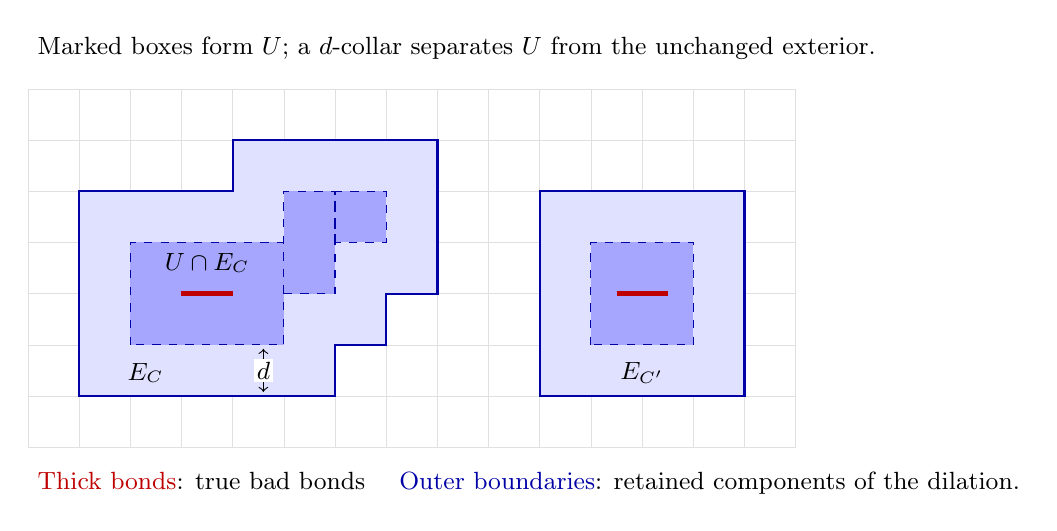
\begin{tikzpicture}[x=0.65cm,y=0.65cm,font=\small]
  \draw[step=1,black!12,very thin] (0,0) grid (15,7);
  \fill[blue!12] (1,1) -- (6,1) -- (6,2) -- (7,2) -- (7,3) -- (8,3) -- (8,6)
      -- (4,6) -- (4,5) -- (1,5) -- cycle;
  \draw[blue!65!black,thick] (1,1) -- (6,1) -- (6,2) -- (7,2) -- (7,3) -- (8,3)
      -- (8,6) -- (4,6) -- (4,5) -- (1,5) -- cycle;
  \fill[blue!35] (2,2) rectangle (5,4);
  \fill[blue!35] (5,3) rectangle (6,5);
  \fill[blue!35] (6,4) rectangle (7,5);
  \draw[blue!65!black,dashed] (2,2) rectangle (5,4);
  \draw[blue!65!black,dashed] (5,3) rectangle (6,5);
  \draw[blue!65!black,dashed] (6,4) rectangle (7,5);
  \fill[blue!12] (10,1) rectangle (14,5);
  \draw[blue!65!black,thick] (10,1) rectangle (14,5);
  \fill[blue!35] (11,2) rectangle (13,4);
  \draw[blue!65!black,dashed] (11,2) rectangle (13,4);
  \draw[red!75!black,line width=2pt] (3,3) -- (4,3);
  \draw[red!75!black,line width=2pt] (11.5,3) -- (12.5,3);
  \node at (2.3,1.45) {$E_C$};
  \node at (12,1.45) {$E_{C'}$};
  \node at (3.5,3.6) {$U\cap E_C$};
  \draw[<->] (4.6,1.08) -- (4.6,1.92);
  \node[fill=white,inner sep=1pt] at (4.6,1.5) {$d$};
  \node[anchor=west,align=left] at (0,7.8)
      {Marked boxes form $U$; a $d$-collar separates $U$ from the unchanged exterior.};
  \node[anchor=west] at (0,-0.7)
      {\textcolor{red!75!black}{Thick bonds}: true bad bonds \quad
       \textcolor{blue!65!black}{Outer boundaries}: retained components of the dilation.};
\end{tikzpicture}
\caption{Schematic editable regions. Each dark region is a union of
marked boxes, and each light region is the complete connected component
of its $d$-dilation. The replacement uses all sites of a selected light
region. Its outer collar lies outside $U$, so it joins the unchanged
configuration without creating a bad bond. Distinct retained components
have nonadjacent sites. The drawing suppresses lattice boundary
conventions and is not to scale.}
\label{fig:editable}
\end{figure}
